\section{JUSTIFICACIÓN TEÓRICA}
%https://www.thetechedvocate.org/8-ways-machine-learning-will-improve-education/
%En primer lugar, y, antes de comenzar la investigación, se ha acudido a los datos del INE (Instituto Nacional de Estadística) y a los del ministerio de educación, ciencia y deportes (MECD).
%Como la investigación va dirigida a los alumnos de la ESO, se ha buscado información respectiva a este nivel educativo. 
En primer lugar, esta investigación se realiza con el propósito de aportar conocimiento existente sobre la importancia de determinadas variables educativas y su relevancia en la predicción en la planificación y la gestión educativa.

En la actualidad existen numerosos informes acerca del uso de la ciencia de datos y sus técnicas en el ámbito educativo. Para la realización de este TFM se han analizado distintas publicaciones de la base de datos científica de ScienceDirect. Para realizar la búsqueda se han utilizado las siguientes palabra claves: educational, data y mining. Se debe recordar que el éxito de la búsqueda depende de estas palabras claves.

De la búsqueda anterior se han obtenido 160 artículos. Posteriormente se han seleccionado aquellos de los últimos 4 años (2016,2017,2018 y 2019). De esta forma obtenemos resultados actuales. Filtrando por fechas, hemos conseguido reducir los resultados a 73 artículos. Se ha realizado una observación sobre los artículos obtenidos y se ha comprobado la existencia de artículos que no resultaban útiles en esta investigación. Por tanto, se ha realizado otra búsqueda utilizando las claves anteriores y añadiendo la clave "prediction". Esta vez, se han obtenido 26 resultados. De todos los resultados obtenido, se han seleccionado 15 artículos que se consideran útiles y que servirán de ayuda.

Debemos destacar que la mayoría de los resultados obtenidos tratan de artículos centrados en la predicción de los resultados académicos del alumnos teniendo en cuenta ciertos factores internos (como las propias calificaciones a lo largo del curso) y externos (como factores etnograficos, edad, situación económica familiar, etc).

En este sentido es interesante realizar un análisis de dichos artículos, puesto que en primer lugar se deberá tener en cuenta cuales son las metodologías de la ciencia de datos que se están utilizando. Ademas, en segundo lugar, se debe tener en cuenta los modelos que se utilizan para predecir variables de carácter educativo. 

Una vez que se han analizado los artículos, se ha decido realizar otra búsqueda en ScienceDirect, teniendo en cuenta las palabras claves: "gis", "data", "mining" y "education". De esta búsqueda se han obtenido 22 resultados. De estos resultados se ha analizado un único articulo que se considera importante. El motivo de esta búsqueda es intentar encontrar artículos centrados en GIS (Sistemas de Información Geográfica). Los sistemas de información geográfica, como su propio nombre indica, se utilizan para referenciar datos en el espacio.

En el artículo de prensa de \citeA{FERNANDES2019335}, se muestra el uso de técnicas como los métodos de clasificación y el algoritmo predictivo de GBM (Gradient Boosting Model) con el objetivo de obtener aquellas variables en el entorno del alumno, que hace que este obtenga mejores o peores resultados escolares. Este estudio, además, tiene el objetivo de aportar información útil para los representantes políticos en el ámbito educativo, el consejo escolar y los profesores con el objetivo de que estos puedan realizar políticas públicas, materiales didácticos y trabajo social para beneficiar a los estudiantes.

Los datos escolares a estudiar proceden de alumnos de colegios de un Distrito Federal de Brasil durante el 2015 y el 2016. Estos datos se han obtenido a partir de la base de datos de iEducar que contiene atributos relacionados con cada alumno. 

Algunas de las variables que se estudian en el articulo anterior pertenecen concretamente al ámbito personal, social y geográfico del alumno. Estas variables son:
\begin{multicols}{2}
\begin{enumerate}[itemsep=0mm]
\item El barrio del alumno.
\item El centro educativo.
\item La edad del alumno.
\item Los ingresos del alumno.
\item Los alumnos con necesidades especiales.
\item El genero. 
\item El entorno en el aula.
\end{enumerate}
\end{multicols}

En esta investigación se utiliza la metodología CRISP-DM (del inglés Cross Industry Standard Process for Data Mining) que es una metodología frecuente en el desarrollo de proyectos de Data Mining. Esta metodología indica cómo debe realizarse el proceso de "data mining". Esta metodología se ha utilizado en otros artículos como \citeA{DELEN2010498} o \cite{SEN20129468}.

Según este mismo artículo de \citeA{SEN20129468}, esta metodología contiene las siguientes fases en el ciclo:
\begin{enumerate}
	\item Entendimiento del negocio. Debe comprenderse los objetivos del negocio. Se debe realizar una descripción del problema. Por ultimo debe hacerse un plan de proyecto para alcanzar los objetivos deseados.
	\item Entendimiento de los datos. Debe identificarse las fuentes de los datos y obtener aquellos datos relevantes para la consecución de los objetivos.
	\item Preparación de los datos. Conlleva el pre-procesado, la limpieza y la transformación de los datos relevantes con el objetivo de usar algoritmos de minería de datos.
	\item Construcción del modelo. Se debe desplegar un gran número de modelos y quedarse con aquellos que devuelvan valores óptimos para los datos utilizados.
	\item Evaluación y Test. Debe evaluarse y probarse los modelos. Deben compararse entre sí y comprobar que son útiles para los datos expuestos.
	\item Puesta en marcha. Realizar actividades usando los modelos seleccionados en el proceso de la toma de decisión.
\end{enumerate}

En la figura \ref{fig:cicloCrisp}, obtenida del artículo de \citeA{SEN20129468} se muestra el ciclo de CRISP.

\begin{figure*}[htb]
	\centering
	\caption{Ciclo de la metodología CRISP}
	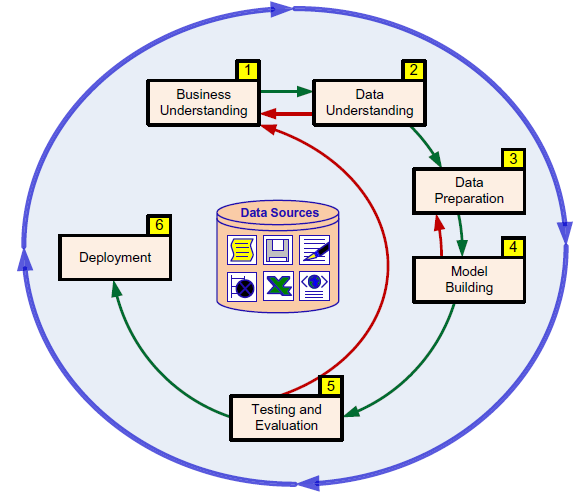
\includegraphics[width=0.6\textwidth]{recursos/CRISPCiclo}
	\label{fig:cicloCrisp}
\end{figure*}


Para realizar la parte de predicción, utiliza las variables anteriormente comentadas, incluidas en dos conjuntos de datos. En el primer conjunto de datos (DS-I), se almacenan los datos obtenidos antes de comenzar el comienzo del año escolar. El segundo conjunto de datos incluye las variables del primer conjunto de datos y alguna nueva que se ha obtenido después del segundo mes del año escolar. Siendo algunas de estas variables nuevas las asignaturas, las notas y las ausencias. Estas dos últimas variables son las que mayor importancia tienen en la revelación de los resultados académicos finales.

El primer conjunto de datos (DS-I) se usa para entrenar el modelo de clasificación I (CM-I), que identifica la probabilidad que tiene un alumno de suspender teniendo en cuenta los datos del comienzo de curso. El segundo conjunto de datos (DS-II) se usa para entrenar el modelo de clasificación II, que también identifica la probabilidad que tiene un alumno de suspender teniendo en cuenta los datos del comienzo de curso e incluyendo las nuevas variables. Una vez que se han entrenado los modelos, se ha utilizado la matriz de confusión para obtener la bondad o efectividad del modelo respecto al conjunto de datos. Los datos obtenidos han mostrado que las variables de ``vecindario", ``colegio", ``ciudad'' y ``edad" son factores relevantes que afectan a los resultados académicos de los alumnos.

Como conclusión, se indica en esta investigación que el entorno social y sus variables tienen una influencia directa en el proceso de enseñar-aprender. Esta investigación puede aportar información a los profesionales que busquen herramientas o métodos para mejorar los resultados escolares de los alumnos.

Por otro lado, en el artículo de prensa de \citeA{ASIF2017177} se citan otras investigaciones realizadas, donde también se utilizan variables sociales como la edad, sexo, nacionalidad, estado civil, desplazamiento (si el alumno vive fuera del distrito), necesidades especiales, tipo de admisión, situación laboral, situación económica, etc.

En el artículo de \citeA{ASIF2017177}, se analiza el rendimiento de los alumnos matriculados en el 4 año del grado universitario de Tecnología Informática. El objetivo es, nuevamente, obtener información sobre el rendimiento de estudiantes para que las personas interesadas (directores y docentes) puedan mejorar el programa educativo. Los enfoques para lograr este objetivo son los siguientes:

\begin{enumerate}
\item En primer lugar se generan clasificadores para predecir el rendimiento de los estudiantes al final del curso académico tan pronto como sea posible. Estos clasificadores toman las calificaciones de admisión y las calificaciones finales del primer y segundo año. No se consideran características socio-económicas o demográficas.
\item En segundo lugar, utilizando estos clasificadores, el objetivo es utilizar cursos que puedan servir como indicadores efectivos del desempeño de los estudiantes. De esta forma se puede ayudar o estimular a los alumnos en riesgo.
\item Por último, se va a investigar como el rendimiento académico progresa sobre el cuarto año del grado. Para ello, se va a utilizar técnicas de \textit{clustering} y se van a dividir a los alumnos en grupos, donde los alumnos de un mismo grupo van a tener la misma progresión en el rendimiento. De esta forma, se van a agrupar los alumnos que hayan tenido bajas calificaciones a lo largo de sus estudios y aquellos que han tenido altas calificaciones a lo largo de sus estudios. La clave es obtener y comprender los indicadores propuestos en el segundo paso.
\end{enumerate}

Los datos utilizados en este articulo proceden de las calificaciones del cuarto año del grado de ingeniería de Tecnología Informática de una universidad de Pakistán. Se van a tomar 210 alumnos que se han matriculado en los cursos de 2007-2008 y 2008-2009. Los datos contienen variables relacionadas con las calificaciones de pre-admisión de los alumnos y de las calificaciones de estos en los siguientes 4 años del programa de grado.
Por tanto, para lograr los objetivos establecidos, \citeA{ASIF2017177}, va a utilizar los arboles de decisión y clúster como técnicas de minería de datos.

Otro de los artículos que se ha utilizado como referencia ha sido el de \citeA{SHAHIRI2015414}. En este artículo, nuevamente se han utilizado técnicas predictivas para la mejora del rendimiento académico de los alumnos. En este caso, los datos utilizados proceden de instituciones malayas. De nuevo se han tenido en cuenta los resultados académicos internos como las calificaciones de prácticas o tareas, exámenes, actividades en el laboratorio, test de clase y atención. También se ha tenido en cuenta factores externos como el género, la edad, el entorno familiar y la discapacidad. Este articulo sirve de referencia para obtener y acotar los modelos a utilizar en este TFM.

En este artículo se indica que ``a priori", sin tener en cuenta la experiencia, es necesario realizar un proyecto piloto, que responda a dos preguntas en concreto. La primera pregunta que se plantea son los atributos o variables a utilizar en la investigación. La segunda pregunta planteada es sobre los métodos predictivos a utilizar. La siguiente figura \ref{fig:precMet} obtenida del artículo, muestra la precisión en la predicción de los algoritmos entre los años 2002 y 2015.

\begin{figure*}[htb]
	\centering
	\caption{Predicción en la precisión agrupada por algoritmos desde 2002 a 2015}
	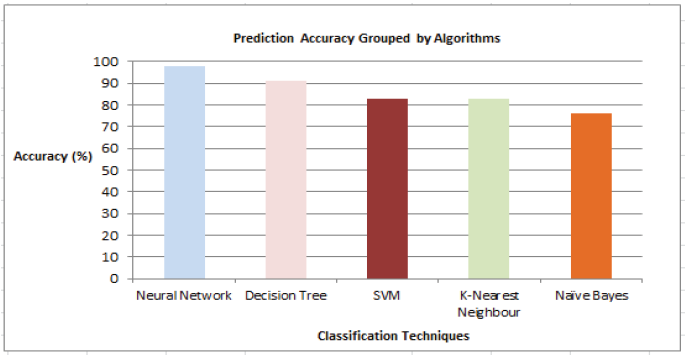
\includegraphics[width=0.8\textwidth]{recursos/PrecisionMetodos}
	\label{fig:precMet}
\end{figure*}

Teniendo en cuenta dicha figura, vemos que las redes neuronales son las que obtienen mejores resultados junto con los arboles de decisiones, lo que significa que se ajustan más a los datos. 

Los resultados obtenidos en otro artículo, concretamente el de \citeA{ASHRAF20181021} indican que el mejor modelo para los datos propuestos ha sido obtenido utilizando el algoritmo de bosques aleatorios. Este algoritmo ha obtenido mejores resultados que otros algoritmos como los arboles de decisión o árbol aleatorio. Este articulo utiliza también datos académicos de alumnos, en este caso, pertenecientes a la Universidad Kashmir.

Una vez que se ha realizado un análisis sobre la metodología utilizada y los algoritmos predictivos, además de tener en cuenta las variables utilizadas (relacionadas con el entorno del alumno), se va a realizar una investigación sobre nuevas variables que podrían incluirse en este TFM.

En el libro de \citeA{PANAHI2019161}, se ha realizado una serie de investigaciones cuyo objetivo ha sido determinar la idoneidad de construir o emplazar centros educativos según pesos dados a factores. Estos factores son los siguientes:

\begin{itemize}
	\item \textbf{Facilidades Urbanas:} En este punto se incluyen las gasolineras, las tuberías de gas de alta presión y las líneas de alta tensión. Cuanto más cerca estén los centros de estas zonas, más riesgo existe para los alumnos. Se tiende por tanto a alejar los centros de estos puntos.
	\item \textbf{Densidad de población y áreas residenciales:} La proximidad de los colegios a zonas residenciales con una gran población de estudiantes es importante, puesto que, a menor distancia entre los estudiantes, los colegios y sus casas menor es el gasto de las familias y menor es la probabilidad de que los alumnos sean secuestrados.
	\item\textbf{ Accesibilidad a red de carreteras urbanas:} La distancia de las calles y las autovías es otro factor importante para situar los colegios. Cuanto más cerca estén los colegios a estas vías, más facilidades tendrán los alumnos, y por lo tanto más ahorro de tiempo y costes.
	Sin embargo, la cercanía de los colegios a las autovías o autopistas, puede implicar mayor riesgo de accidentes. Sin embargo, si las autovías o autopistas se encuentran lejos, se reduce la accesibilidad a los colegios. Es necesario situar los centros en puntos intermedios (100-200m).
	\item \textbf{Servicios Urbanos:} Las distancias a los hospitales, a las estaciones de bomberos y de policía tienen mayor influencia. Sin embargo, estos deben situarse a distancias prudenciales de los centros (100-200m).
	\item \textbf{Centros culturales:} La proximidad de los centros culturales incrementa la salud espiritual y psicológica del alumno, incrementando así sus conocimientos. Curiosamente, si existen estos tipos de centros cercanos al colegio, entonces no es necesario que dichos colegios dispongan de estos servicios (pudiéndose ampliar las aulas, el comedor, etc)
\end{itemize}                     

La investigación se ha llevado a cabo en la ciudad de Tehran. Se han tomado para el estudio dos distritos. Uno de ellos contiene 106 colegios y el otro 137. A partir de la geolocalización de dichos colegios y de los subfactores comentados, se ha realizado un estudio sobre la relación existente entre los factores y subfactores y los colegios.

Los pesos dados a cada factor y subfactor se han determinado utilizando un algoritmo llamado SWARA. Los resultados finales obtenidos indican que existen subfactores que influyen más o menos en la posición del centro.

Por tanto, una vez que se ha estudiado una metodología de trabajo, y se han observado un gran número de variables relacionadas con los alumnos y con los centros, además de haber agrupado ciertos algoritmos que pueden aportar mayor información sobre los datos educativos, se va a realizar la investigación propia para resolver el problema propio de este TFM.




%manage, education, data mining -> Castilla y Leon
%GIS-Based SWARA and Its Ensemble by RBF and ICA Data-Mining Techniques for Determining Suitability of Existing Schools and Site Selection of New School Buildings


